
\documentclass[10pt]{standalone}
\input{../tikzpic_packages.tex}
\begin{document}
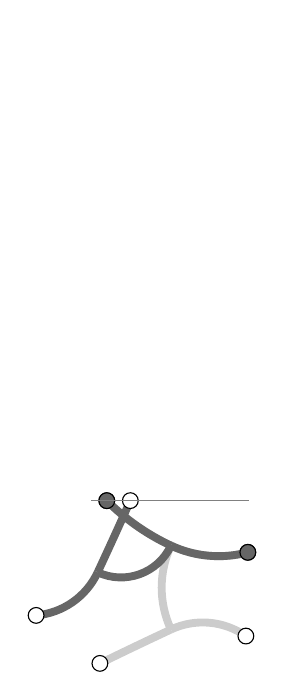
\begin{tikzpicture}
\tikzset{
    part/.style={line width = 1mm, color=\col},
    foot/.style={fill=white},
    footfixed/.style={fill=\col},
    grid line/.style={white},
    start line/.style={help lines}}
\def\rfoot{.1}

\foreach \y in {0,1,2,3,4,5,6,7,8}{
    \draw[grid line] (0.000000, 2.000000)++(-.2,-2+\y)--++(2,0);
}
\foreach \x in {0,1,2}{
    \draw[grid line] (0.000000, 2.000000)++(-.2+\x,-2)--++(0,8);
}
\draw[start line] (0.000000, 2.000000)++(-.2,0)--++(2,0);

\def\col{black!20}
\def\alpi{20.000000}
\def\beti{40.000000}
\def\gam{50.000000}
\def\alpii{1.000000}
\def\betii{60.000000}
\def\gamh{25.000000}

\def\eps{90.000000}
\def\ci{45.000000}
\def\cii{105.000000}
\def\ciii{296.000000}
\def\civ{235.000000}

\def\ri{2.864789}
\def\rii{1.432394}
\def\rg{1.260507}
\def\riii{57.295780}
\def\riv{0.954930}

\path (0.000000, 2.000000)coordinate(F1);

\draw[part] (F1)arc(180+\ci:180+\ci+\alpi:\ri)coordinate(OM);
\draw[part] (OM)arc(180+\ci+\alpi:180+\ci+\alpi+\beti:\rii)coordinate(F2);
\draw[part] (OM)arc(90+\ci+\alpi:90+\ci+\alpi+\gam:\rg)coordinate(UM);
\draw[part] (UM)arc(\gam+\ci+\alpi:\gam+\ci+\alpi+\alpii:\riii)coordinate(F3);
\draw[part] (UM)arc(\gam+\ci+\alpi:\gam+\ci+\alpi-\betii:\riv)coordinate(F4);

\draw[footfixed] (0.000000, 2.000000)circle(\rfoot);
\draw[foot] (1.791087, 1.343935)circle(\rfoot);
\draw[foot] (-0.087574, -0.066601)circle(\rfoot);
\draw[foot] (1.766295, 0.280677)circle(\rfoot);

\def\col{black!60}
\def\alpi{20.000000}
\def\beti{40.000000}
\def\gam{-90.000000}
\def\alpii{1.000000}
\def\betii{60.000000}
\def\gamh{-45.000000}

\def\eps{20.000051}
\def\ci{45.000051}
\def\cii{105.000051}
\def\ciii{156.000051}
\def\civ{95.000051}

\def\ri{2.864789}
\def\rii{1.432394}
\def\rg{-0.700282}
\def\riii{57.295780}
\def\riv{0.954930}

\path (0.000000, 2.000000)coordinate(F1);

\draw[part] (F1)arc(180+\ci:180+\ci+\alpi:\ri)coordinate(OM);
\draw[part] (OM)arc(180+\ci+\alpi:180+\ci+\alpi+\beti:\rii)coordinate(F2);
\draw[part] (OM)arc(90+\ci+\alpi:90+\ci+\alpi+\gam:\rg)coordinate(UM);
\draw[part] (UM)arc(\gam+\ci+\alpi:\gam+\ci+\alpi+\alpii:\riii)coordinate(F3);
\draw[part] (UM)arc(\gam+\ci+\alpi:\gam+\ci+\alpi-\betii:\riv)coordinate(F4);

\draw[footfixed] (0.000000, 2.000000)circle(\rfoot);
\draw[footfixed] (1.791087, 1.343936)circle(\rfoot);
\draw[foot] (0.299065, 2.000562)circle(\rfoot);
\draw[foot] (-0.897854, 0.542886)circle(\rfoot);

\draw[start line] (0.000000, 2.000000)++(-.2,0)--++(2,0);
        
\end{tikzpicture}
\end{document}
